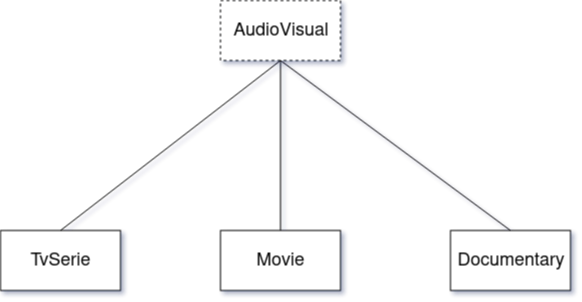
\includegraphics[width=1\textwidth]{gerarchia}
\paragraph{Gerarchia dei tipi}
La gerarchia è così composta: una classe base astratta denominata \textit{AudioVisual}, tre classi derivate \textit{TvSerie}, \textit{Movie}, \textit{Documentary} che implementano i metodi puri della classe base. \newline

\paragraph{AudioVisual}
I campi dati sono:
\begin{itemize}
    \item Title
    \item Description
    \item ReleaseDate
    \item RunningTime
    \item Director
    \item Favorite
    \item Audio
    \item Video %4k, 144p, 240, 480, 360, 720
%4k/2160p, FullHD/1080p, HD/720p, SD/480p, LD/240p
%fps frame per secondo
    \item Pic %immagine di copertina
% lingua originale, sottotitoli
\end{itemize}
I metodi sono:
\begin{itemize}
    \item Costruttore
    \item Distruttore
    \item Clone : metodo usato da deepptr per la costruzione di copia profonda
    \item Operatore di uguaglianza e disuguaglianza
    \item isFavorite : metodo usato per sapere se un "AudioVisual" è tra i preferiti dell'utente
    \item getTotalRunningTime : metodo che restituisce il tempo totale di un AudioVisual o sotto tipo
    \item getType : restituisce il tipo dell'oggetto d'invocazione ("tipo")
    \item getQuality : Audio + Video % se definisco dei range diversi per ogni sottotipo allora questo metodo è virtuale puro
    \item get : genere + rating 
\end{itemize}

\paragraph{TvSerie}
I campi dati sono:
\begin{itemize}
    \item Season
    \item Episode
    \item Cast
    \item Genre 
    \item Rating 
    \item Ended 
\end{itemize}
I metodi sono:
\begin{itemize}
    \item implementa i metodi virutali puri della classe base astratta AudioVisual
\end{itemize}

\paragraph{Movie}
I campi dati sono:
\begin{itemize}
    \item Cast
    \item Genre
    \item Rating
    \item Collection 
\end{itemize}
I metodi sono:
\begin{itemize}
    \item implementa i metodi virutali puri della classe base astratta AudioVisual
    \item isCollection
\end{itemize}

\paragraph{Documentary}
I campi dati sono:
\begin{itemize}
    \item Narrator
    \item Topic : si spazia da argomento scientifico, storico a quelli biografici
\end{itemize}
I metodi sono:
\begin{itemize}
    \item implementa i metodi virutali puri della classe base astratta AudioVisual
\end{itemize}

\paragraph{User}
I campi dati sono:
\begin{itemize}
    \item Nickname
    \item TotalTime
\end{itemize}
I metodi sono:
\begin{itemize}
    \item getTotalTime : somma di tutti i RunningTime degli AudioVisual appartenenti alla lista
\end{itemize}
